L’étude des logiciels développés ou utilisés par les économistes-programmeurs met en évidence un processus récurrent : leur conception naît presque toujours de la rencontre entre un besoin scientifique concret et des compétences techniques acquises, souvent de manière autodidacte. Chaque programme répond d’abord à une finalité précise, qu’il s’agisse de simplifier un travail, de rendre une méthode accessible ou d’explorer un phénomène difficile à appréhender par d’autres moyens. Certains de ces logiciels ont ensuite connu une diffusion élargie, au point de transformer durablement certaines pratiques de la discipline. L’analyse qui suit porte principalement sur ces cas de réussite, puisque ce sont ceux qui ont laissé une trace visible. Elle ne doit toutefois pas oublier l’existence très probable de nombreux projets avortés ou demeurés confidentiels, qui témoignent aussi des contraintes techniques et institutionnelles pesant sur l’informatisation du travail économique, et qu'il faudrait étudier dans un autre travail.

Genèse et fonctions des logiciels


\textbf{PcGive / OxMetrics (David Hendry, Jurgen Doornik)}

L’histoire de PcGive commence avec la fin des ordinateurs mainframe. Durant son doctorat à la LSE, Hendry contribue au développement de la bibliothèque de programmes Autoreg. Suite à son doctorat Hendry rejoint Oxford pour son premier poste de Professeur et y découvre les premiers PC, des ordinateurs personnels et avec un écran permettant d'avoir un retour immédiat sur les actions qu'on y fait. A comparer au mainframe et aux retours sous formes feuilles de papiers imprimés. Hendry, convaincu de l'importance et de la pertinence des écrans pour la pratique de l'économétrie, entreprend alors de réécrire la bibliothèque Autoreg pour pouvoir l'utiliser sur un PC. Cette bibliothèque de programmes prend alors la forme d'un grand volume de cartes perforées en carton. Hendry passera trois années à la retranscrire sur PC.
PcGive, dont la première version date de 1984, est ainsi conçu comme un logiciel scientifique et pédagogique, composé d'un ensemble de sous-routines permettant l’estimation d’un large éventail de modèles économétriques, la réalisation de simulations par méthode de Monte Carlo et la génération de données. PcGive introduit une interface guidée par menus, permettant aux étudiants comme aux chercheurs d’explorer différentes procédures économétriques sans avoir à écrire eux-mêmes le code permettant d'effectuer ces calculs. Le logiciel vise explicitement à transformer l’enseignement, en donnant la possibilité de faire des démonstrations, devant les étudiants, de l’effet d’un modèle mal spécifié ou d’un changement structurel sur les résultats obtenus à l'écran.
L’évolution technique du projet est marquée par la rencontre avec Jurgen Doornik, qui assure la réécriture du système en C et introduit le langage Ox. Celui-ci offre une souplesse inédite : le code généré automatiquement par PcGive peut être sauvegardé et réutilisé comme script indépendant, garantissant à la fois la reproductibilité et l’extensibilité des analyses. Autour de Hendry et Doornik se constitue une véritable équipe de développeurs (Hans-Martin Krolzig pour PcGets, Siem Jan Koopman pour STAMP, Sebastien Laurent pour G@rch), donnant naissance à une suite logicielle complète, connue sous le nom d’OxMetrics.



\textbf{WinSolve (Richard Pierse)}

Dans un autre registre, WinSolve témoigne de l’importance des logiciels dans la modélisation macroéconomique. Ce logiciel est né de la volonté politique de Jeremy Bray, un membre du parlement très intéressé par les sujets macroéconomiques. En 1994, Bray pose un constat, les outils informatiques utilisés dans les différentes institutions du Royaume-Uni faisant des projections macroéconomiques (le Trésor, la Banque centrale, l'institut national de la statistique, notamment) sont très divers et anciens. Il décide donc de pousser l'Economic and Social Research Council (ESRC), un organisme public du Royaume-Uni dont la mission est de financer les recherches en sciences sociales et ayant financé beaucoup de prévisions macroéconomiques à cette époque, à lancer un appel à candidature. L'objectif de ce projet est de financer le développement d'un logiciel à l'état de l'art, qui serait ensuite utilisé par tous les acteurs de la prévision bénéficiant de financement de l'ESRC. Cependant le public visé par ce logiciel s'oppose à ce projet. Les financements de l'ESRC s'étant taris quelques années avant, ces chercheurs financent leurs travaux en vendant leurs projections, en se différenciant notamment par leurs logiciels. Malgré cette opposition, l'appel à candidature est lancé et c'est Pierse qui le remporte. Il créer donc WinSolve, et décide d'adopter pour ce faire, le langage C++, à la pointe pour le développement d'applications sur Windows, le système d'exploitation le plus répandu à cette époque. Le logiciel permet notamment de résoudre numériquement des modèles non linéaires, d’incorporer des anticipations rationnelles et de tester rapidement différents scénarios contrefactuels. Le public ciblé initialement par le projet n'adopte pas WinSolve, pour les raisons citées précédemment, mais celui-ci trouvera son public, notamment au sein de plusieurs banques centrales à travers le monde.

Il est important de noter que c'est le seul logiciel étudié dans ce mémoire, qui est né d'une commande, d'un appel à projet précis. Sugarscape a également bénéficié d'un financement dès sa création, mais l'objectif du projet était très ouvert car exploratoire, et c'est grâce à cette liberté intellectuelle qu'Epstein et Axtell ont donné naissance à l'agent based modelling.



\textbf{z-Tree (Urs Fischbacher, Stefan Schmid)}

Le cas de z-Tree illustre le rôle décisif des trajectoires individuelles et du hasard des opportunités dans la genèse d’un logiciel. Contrairement à l’idée d’un projet réfléchi et confié à un programmeur, l’histoire de z-Tree commence plutôt par une rencontre fortuite : Urs Fischbacher, alors mathématicien de formation sans cursus en économie, et ingénieur logiciel dans une entreprise privée, tombe par hasard sur une annonce d’Ernst Fehr recherchant un programmeur. Lors de l’entretien, Fehr évoque des thématiques comme les jeux de biens publics, qui enthousiasment Fischbacher et l’incitent à rejoindre l'unité de recherche de Ernst Fehr. Sa mission est alors de programmer les expériences du laboratoire, en suivant les descriptions des protocoles d'expérience conçus par les chercheurs. La programmation d'une expérience est alors très chronophage. Fischbacher conçoit z-Tree, un langage de programmation qui doit rendre les expériences plus simples à programmer. z-Tree repose sur une architecture client-serveur permettant de gérer en temps réel des interactions entre plusieurs dizaines de participants, tout en offrant une interface de programmation relativement simple pour les chercheurs. Ce nouvel outil permet de réduire les coûts logistiques et de pouvoir répliquer un même protocole expérimental de nombreuses fois et dans des laboratoires différents, accroissant ainsi la réplicabilité et donc la robustesse de l'économie expérimentale. Le besoin est donc d'abord local, Fischbacher veut simplifier son travail de programmation des expériences. Mais z-Tree acquiert rapidement une portée plus large. Dès 1998, Fischbacher est invité à Berlin pour enseigner son usage, marquant le début de sa diffusion internationale. À partir de là, le logiciel devient progressivement un standard de facto de l’économie expérimentale, contribuant à la professionnalisation et à l’expansion rapide de ce champ. En 2002, un second développeur, Stefan Schmid, ayant fait des études d'informatiques à l'ETH de Zurich est recruté pour seconder Fischbacher dans son travail sur z-Tree.



\textbf{Gambit (Theodore Turocy, Richard McKelvey et Andrew McLennan)}

La création de Gambit, amorcée à la fin des années 1980 par Ricahrd McKelvey et Andrew McLennan, puis reprise et développée par Theodore Turocy, répond à un besoin spécifique de la théorie des jeux : calculer systématiquement des équilibres dans des jeux de plus en plus complexes. McKelvey et McLennan, les deux créateurs de Gambit, ont suivi une formation de mathématiciens, puis se sont tournés vers l'économie et à la théorie du vote via la théorie des jeux. Le logiciel propose une bibliothèque d'outils computationnelle permettant de représenter des jeux en forme normale ou extensive et d’en extraire différents types d’équilibres (Nash exacts ou approximatifs, epsilon-équilibres). Le projet prend corps dans un cadre artisanal, au sein du département d’économie de Caltech. Il mobilise ponctuellement un ou deux étudiants en informatique de Caltech, recrutés comme programmeurs, sur des budgets dont nous ignorons la provenance. Un tournant intervient en 1993, lorsque le projet obtient une subvention de la National Science Foundation (NSF), qui permet d’assurer son développement jusqu’en 1999. C’est dans ce cadre que Turocy entreprend de réécrire Gambit dans le langage C++. Cette transition vers C++ intervient à peu près au moment où Pierse choisit lui aussi C++ pour écrire WinSolve.
Au fil du temps, Gambit va se diffuser hors du cadre confidentiel de Caltech. Certains enseignants se saisissent de son interface graphique pour illustrer leurs cours de théorie des jeux, donnant ainsi une visibilité nouvelle au projet. Theodore Turocy, qui en reprend la direction à la fin des années 1990, contribue à cette ouverture. Il se souvient d’avoir réalisé une démonstration de Gambit lors du premier congrès mondial de la Game Theory Society, organisé à Bilbao en 2000 : un moment à la fois de diffusion du logiciel et d’intégration dans la communauté académique.



\textbf{Sugarscape (Joshua Epstein et Robert Axtell)}

Sugarscape est un modèle de simulation basé sur des agents. Il simule une société d'agents interagissant sur une grille où les ressources, comme le "sucre", sont inégalement distribuées. Les agents suivent des règles simples\footnote{"Règles définis par l'utilisateur et qui changent en fonction des comportements auxquels on s'intéresse"} (se déplacer, consommer, échanger) pour survivre, ce qui permet d'observer des phénomènes émergents complexes comme l'inégalité économique, les migrations ou les conflits. Développé au Santa Fe Institute, Sugarscape a influencé les études en sciences sociales computationnelles en démontrant comment des comportements collectifs émergent d'interactions individuelles. Cette logique ressemble beaucoup au "Jeu de la vie" de Conway ou au modèle de Schelling, mais Epstein, dans son entretien \cite{epsteinInterviewJoshuaEpstein2024} à la page 2, affirme ne pas avoir eu connaissances de ses travaux lors de la conception de Sugarscape.
L’idée de ce modèle conçu en 1991 au Brookings Institution par Joshua Epstein et Robert Axtell, dans le cadre du 2050 Project financé par la Fondation MacArthur et en lien avec le Santa Fe Institute, apparait au cours d’une discussion à la cantine. Il s’agit alors d’esquisser « la société la plus simple possible que l’on puisse modéliser informatiquement » : un paysage de ressources, des agents dotés d’une vision et d’un métabolisme, se déplaçant pour survivre et interagir. Les interlocuteurs dessinent un schéma de leurs réflexions sur une serviette de la cantine. Cette serviette est conservée par Axtell qui la présente pendant son entretien pour le projet \textit{Oral History of Economics}\cite{axtellInterviewRobertAxtell2025} :

\begin{figure}[h]
  \centering
  \includegraphics[width=0.8\textwidth]{figures/napkinSugarscape.pdf}
  \caption{Le schéma du modèle Sugarscape sur une serviette en papier}
  \label{fig:graph_napkin_Sugarscape}
\end{figure}


À partir de cette base minimale, le modèle est progressivement enrichi — reproduction, transmission culturelle, échanges commerciaux ou dynamiques épidémiques — afin d’explorer comment des règles élémentaires peuvent engendrer des structures sociales complexes. Beaucoup d'applications possibles sont décrites par Epstein et Axtell dans leur livre \cite{epsteinGrowingArtificialSocieties1996}. Cette publication fait de Sugarscape un jalon fondateur de la modélisation basée sur les agents. Bien que critiqué pour la simplicité de ses hypothèses, il ouvre un espace heuristique inédit et suscité de nombreuses applications allant de l’économie à l’épidémiologie, en passant par la science politique et l’archéologie.



\textbf{Le cas particulier d’Agnès Gramain}

À la différence de ses collègues, Gramain ne conçoit pas de logiciel original destiné à la diffusion. Son apport réside dans un usage intensif de logiciels existants (SAS, GAUSS) qu’elle adapte à ses besoins, notamment pour de l'analyse micro économétrique.



%----------------------------------------------------------------------------------------
%	SECTION 1
%----------------------------------------------------------------------------------------

\section{Des logiciels issus de besoins locaux}


L’analyse de ces logiciels révèle un trait marquant : à l’exception notable de WinSolve, tous sont développés en réponse à un besoin local. 

z-Tree est conçu par Urs Fischbacher avant tout pour simplifier son propre travail de programmation des protocoles expérimentaux dans le laboratoire d’Ernst Fehr ; Gambit apparaît à Caltech pour automatiser le calcul d’équilibres de Nash dans des jeux de plus en plus complexes ; quant à David Hendry, il regroupe dans PcGive les routines qu’il utilisait sur mainframe à la LSE, afin de les rendre utilisables sur PC lors de son arrivée à Oxford. 

Le cas de Sugarscape est un peu différent, puisqu’il ne vise pas à faciliter une tâche déjà existante, mais inaugure une nouvelle approche méthodologique — la modélisation basée sur les agents (agent-based modeling, ABM). 
La commande de la Fondation MacArthur dans le cadre du 2050 Project est un peu flou. L’idée initiale de « prendre un regard d’ensemble sur la soutenabilité mondiale », laisse une grande liberté aux chercheurs sur les méthodes à adopter. Confrontés à cette mission, Epstein et Axtell imaginent une « artificial social life » modélisée sur ordinateur. Ici, le besoin local n’est pas celui d’un chercheur face à une contrainte méthodologique immédiate, mais la rencontre de philantropes cherchant à stimuler une recherche prospective et de chercheurs disposant des compétences techniques nécessaires pour inventer une nouvelle manière de représenter des dynamiques sociales complexes.


Seul WinSolve se distingue nettement de cette logique : il est conçu dans le cadre d’un appel à projets de l’ESRC, avec un cahier des charges explicite, un public cible identifié et l’ambition d’harmoniser les pratiques de modélisation macroéconomique d’un ensemble d’institutions britanniques.

Dans l’ensemble, aucun de ces logiciels n’a été conçu initialement comme un produit destiné à être diffusé commercialement ou reconnu académiquement à grande échelle. Leur genèse procède d’abord de la résolution de problèmes immédiats, rencontrés par les chercheurs dans leurs pratiques professionnelles. Ce trait commun leur confère un air de « bricolage », au sens où la conception logicielle relève moins d’un plan stratégique que d’une accumulation de petites décisions et d’arrangements pragmatiques. Comme le montre également l’histoire de Dynare, analysée par \cite{cherrierWriteYourModel2023}, de nombreux logiciels en économie partagent ce même profil : conçus pour répondre à un problème local, ils sont ensuite stabilisés et diffusés au-delà du cercle de leurs créateurs.

Cette logique de la « débrouillardise » n’est pas anodine. Elle éclaire à la fois la force et la fragilité de ces logiciels. Leur force tient à leur pertinence immédiate : conçus pour résoudre une contrainte concrète, ils apportent une solution efficace et directement opérationnelle. Leur fragilité vient du fait que cette conception sous forme de bricolage atteint vite ses limites lorsque le projet se développe. De plus, l'ingénierie logicielle étant une activité très chronophage et requérant un haut niveau d'expertise technique élevé, la maintenance de ces logiciels engendre des coûts élevés. Enfin, comme mentionné dans le premier chapitre, la difficulté pour les économistes à obtenir une reconnaissance académique pour ce type de contributions n'incitent pas les chercheurs et chercheuses à y consacrer du temps.





\section{Des instruments techniques ou des outils heuristiques}

Comme nous l'avons vu dans la première partie, les logiciels analysés sont souvent des instruments créer pour répondre à un besoin technique. Mais au-delà de la simplification de tâches existantes, deux des logiciels étudiés ouvrent des perspectives inédites en permettant d’explorer des phénomènes qui ne pouvaient pas être abordés auparavant par des moyens traditionnels. Ils ne se contentent pas de remplir des fonctions techniques comme l'automatisation de calculs : ils fonctionnent comme de véritables outils heuristiques, ouvrant de nouveaux paradigmes et stimulant la formulation de nouvelles hypothèses.

Le cas de Sugarscape, développé par Joshua Epstein et Robert Axtell, illustre de manière nette cette capacité heuristique. En simulant une société artificielle minimaliste, le modèle met en scène des agents dotés de règles élémentaires de déplacement et de consommation. Or, en observant l’évolution spontanée du système, les chercheurs découvrent l’apparition d'une distribution de richesse fortement inégalitaire, qui suivent une loi de Pareto. Cet effet, non anticipé par les concepteurs eux-mêmes, constitue un exemple frappant d’auto-organisation : des règles locales très simples suffisent à générer une régularité macroéconomique. De la même manière, des dynamiques de ségrégation spatiale, de transmission culturelle ou encore de propagation épidémique émergent des simulations, ouvrant la voie à une relecture de phénomènes sociaux et économiques bien connus à travers le prisme des ABM. Sugarscape ne se limite donc pas à reproduire des comportements déjà théorisés : il produit de nouvelles régularités, inattendues, qui redéfinissent ce qu’il est possible d’expliquer et d’observer dans un cadre computationnel. Le logiciel devient ainsi un outil d’exploration, révélant comment des comportements macroéconomiques ou sociaux peuvent être générés à partir de règles simples à l'échelle micro.

Le logiciel Gambit accomplit une fonction comparable dans un autre registre : celui de la théorie des jeux. En systématisant les calculs, Gambit permet d’explorer numériquement des jeux de grande taille ou des structures trop complexes pour être traitées à la main. Il rend visibles des solutions qui, faute d’outils computationnels, restaient purement théoriques ou inaccessibles. Ainsi Turocy témoigne par exemple avoir découvert un théorème, qui lui aurait été suggéré par les résultats obtenus avec Gambit. Et il transforme cette preuve du théorème en un article publié dans un journal d'économie. Turocy décrit le champ des possibles ouverts par Gambit en utilisant une métaphore, selon lui, « en économie, la théorie des jeux computationnelle est parfois une réponse en quête d’une question ». 

Dans les deux cas, l’utilisation des logiciels va au-delà de l’exécution automatique d’algorithmes. Ils permettent, par la simulation, de révéler des régularités que ni l’intuition ni le calcul manuel ne permettaient d'anticiper. En ce sens, ces programmes participent à la transformation la pratique économique : ils enrichissent la boite à outils des économistes en devenant de nouveaux critères d’explication en sciences économiques. C'est ici l'informatique qui permet l'apparition de ces nouvelles méthodes de modélisation.

Cependant, que ces logiciels soient nés pour répondre à des contraintes techniques (comme vu dans la première section) ou qu’ils aient ouvert de nouveaux champs d’exploration (comme vu dans cette deuxième section), ils se heurtent aux mêmes difficultés. La maintenance d'un logiciel est chronophage et dispendieuse, et le conservatisme des meilleures revues académiques en économie rend difficile la publication de travaux de recherche centrés sur un logiciel. Nous allons voir dans cette troisième section comment les concepteurs de ces outils se sont adaptés face à ces difficultés.



\section{Financement et reconnaissance}



Si l’on considère les logiciels étudiés, un constat s’impose : trois logiciels apparaissent sans financement spécifique. Gambit, au début des années 1990, est développé par Richard McKelvey et Andrew McLennan sur leur temps de recherche académique, sans autre ressource que leurs salaires universitaires et l’appui occasionnel d’étudiants. 

De même, z-Tree, conçu en 1995 par Urs Fischbacher, est programmé alors que celui-ci est employé par son laboratoire comme technicien : son développement s’inscrit ainsi dans son temps de travail, rémunéré par l’institution, mais sans budget supplémentaire ni projet dédié. 

Et PcGive de Richard Hendry, nait de Autoreg, une bibliothèque constituée de dizaines de sous-routines crées par les économètres de la LSE. Dans les trois cas, le logiciel émerge avant tout grâce à l’investissement individuel des chercheurs, soutenu de manière indirecte par leurs postes universitaires, plutôt que d’un financement explicite destiné à la programmation. 

Seul WinSolve bénéficie d’un financement explicitement dédié au développement d’un logiciel. Cette exception s’explique par l’influence décisive de Jeremy Bray, un membre du Parlement britannique particulièrement engagé dans les questions de prévisions macroéconomiques. Sous son impulsion, l’ESRC met en place un soutien spécifique pour appuyer la réalisation de WinSolve, malgré la désapprobation des institutions auxquelles ce logiciel est destiné. 

Enfin, le cas de Sugarscape est un cas un peu particulier. C'est bien un financement institutionnel, ou philanthropique, de la Fondation MacArthur, dans le cadre du 2050 Project, qui permet sa création par Joshua Epstein et Robert Axtell. Cependant le 2050 Project n'est pas explicitement fléché vers le développement de logiciel, il a pour objectif d'explorer ce à quoi pourrait ressembler le monde en 2050, en particulier sous l’angle des enjeux environnementaux et de durabilité. C'est dans le cadre de ce programme relativement flou et exploratoire qu'Epstein et Axtell disposent d’une liberté de recherche inhabituelle, ce qui permet l'élaboration et la conception d’un logiciel et d'un modèle aussi novateur que Sugarscape. D’après les archives de la Fondation MacArthur \cite{MacArthurG}, le financement initial s’élève à 250 000 dollars en 1992 — soit environ 575 000 dollars de 2025 — répartis sur 4 ans.

\begin{figure}[h]
  \centering
  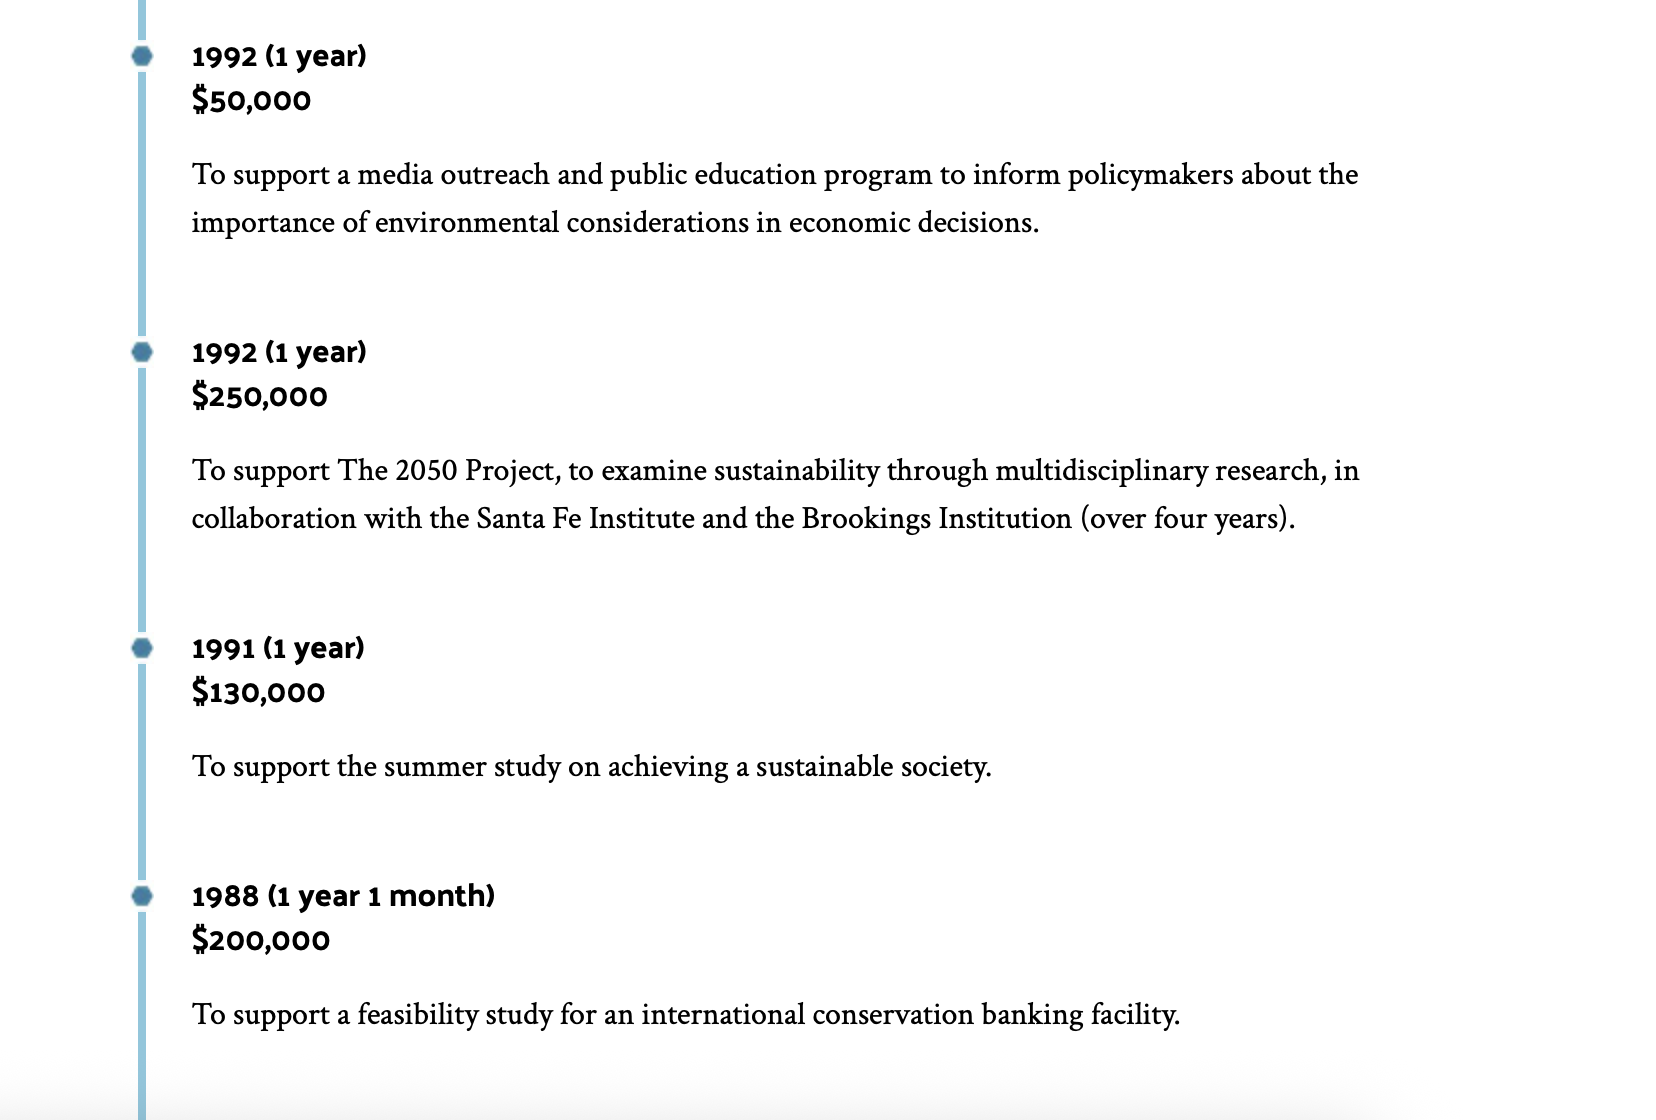
\includegraphics[width=0.8\textwidth]{figures/MacArthur_grants.png}
  \caption{Liste des financements accordés par la MacArthur Foundation sur son site internet}
  \label{fig:graph_grants_Project2050}
\end{figure}


Ce n’est que dans un second temps que certains projets bénéficient de subventions décisives. 

David Hendry explique dans son entretien avoir bénéficié du soutien de l’ESRC pour l’acquisition de son premier ordinateur personnel, et souligne que les financements de recherche en économétrie incluaient presque toujours une composante de développement logiciel, ce dernier étant indispensable à l’avancée de la discipline elle-même, étroitement liée à l’informatique (comme l’a également noté Renfro \cite{renfroEconometricsComputerLove2011} \cite{renfroEconometricSoftwareFirst2004}). Toutefois, aucun de ces financements n'est exclusivement consacré à la création et à la maintenance des logiciels : ils sont intégrés dans des projets de recherche plus larges, dont la programmation constitue une condition nécessaire mais non un objectif en soi.

La National Science Foundation (NSF) finance Gambit entre 1994 et 1999, permettant sa réécriture en C++ et une importante extension de ses fonctionnalités.

Mais si les financements sont déterminants pour le lancement, leur maintien en condition opérationnel, sur le long terme se révèle beaucoup plus difficile. En 1999, lorsque le financement de l’ESRC arrive à son terme, Pierse est poussé par l'institution à commercialiser le logiciel, car elle souhaite voir le logiciel maintenu. WinSolve est alors commercialisé par Timberlake Consultants, une entreprise spécialisée dans la distribution de logiciels dédiés à l'économétrie, la statistique et la prévision. 

La même incitation avait été faite à Hendry quelques années avant, rendant l'utilisation de PcGive payante. 

Gambit connaît un destin encore plus incertain : après la fin du soutien de la NSF, il survit près de vingt ans grâce au volontarisme de Turocy et de quelques collaborateurs, sans véritable financement structuré.  Et le développement du logiciel s’en trouve affecté, comme en témoigne Turocy dans son entretien et comme le montre ce graphique présentant le nombre d’additions et de suppressions de code réalisées dans Gambit au fil des années : on y observe une activité soutenue à la fin des années 1990 et au début des années 2000, suivie de phases de ralentissement, voire de quasi-abandon, avant une reprise en 2021. 

Cette évolution traduit bien le caractère irrégulier et dépendant des disponibilités individuelles du développement du logiciel, plutôt que le développement continu d’un projet durablement financé.

\begin{figure}[h]
  \centering
  \includegraphics[width=0.8\textwidth]{figures/code_frequency_Gambit.png}
  \caption{Évolution de l’activité de développement du logiciel Gambit (1995–2025)}
  \label{fig:graph_commits_Gambit}
\end{figure}

Quant à Sugarscape, le logiciel n'est pas maintenu après la publication des résultats du Project 2050 et du livre \cite{epsteinGrowingArtificialSocieties1996} : le logiciel laisse une trace durable dans la littérature, mais ne connait pas de développement actif. Le concept est cependant repris et développé dans de nombreux logiciels dont les plus connus sont NetLogo, MASON ou Repast.

Dans tous ces cas, la question de la pérennité financière apparaît comme un point de fragilité majeur.

À ces difficultés matérielles s’ajoute le problème de la faible reconnaissance académique. Plusieurs concepteurs soulignent combien il est difficile de publier des articles directement centrés sur le développement ou l’architecture de leurs logiciels. 

Pierse raconte avoir subi une certaine pression de la part de son employeur, l'Université de Surrey, pour limiter son temps de travail sur WinSolve. En effet, ce travail chronophage est quasiment impossible à transformer en publication, ou du moins les revues refuse ses soumissions sur WinSolve, quand bien même l’outil suscite un vif intérêt auprès de ses utilisateurs. 

De même, Fischbacher voit ses soumissions d'articles au journal \textit{Experimental Economics} rejetées, avant que ce même journal accepte de publier un article décrivant z-Tree en 2007, alors même que le logiciel était déjà devenu un standard de facto dans les laboratoires expérimentaux. Cette réticence des revues traduit un biais profond : la programmation est perçue comme un travail technique, auxiliaire de la recherche, et non comme une contribution scientifique en soi.

Le cas de Jurgen Doornik, qui est en charge de la plupart du travail technique sur PcGive et OxMetrics, est particulièrement éclairant : malgré ses contributions majeures — réécriture de l’ensemble des logiciels de David Hendry, création du langage Ox —, Pierse dans son entretien, estime qu'il n'a pas reçu la reconnaissance que mériterait un tel apport :

\begin{quote}
\begin{center}
\textit{"People who were spending a lot of time actually doing programming were not the people who were having great academic careers. I mean, that’s what I sort of observed. People like Jurgen Doornik, for example […] not really had the ... acclaim ... that I think he deserves. […] The top journals won’t ever publish stuff on this sort of thing"}
\end{center}
\end{quote} \hfill Déclaration de Pierse, page 25 de l'entretien pour Oral History of Economics \cite{pierseInterviewRichardPierse2024}



Fischbacher, pour tenter de pallier à cette faible reconnaissance, choisit dès 1997 de diffuser z-Tree sous la forme d’un \textit{citeware}. Ce type de licence impose que toute publication scientifique utilisant le logiciel mentionne explicitement son emploi et cite un article de référence dans la bibliographie. Dans le cas de z-Tree, cet article de référence demeure longtemps un working paper, à cause des difficultés mentionnées ci-dessus à faire publier son travail. Ce n’est qu’en 2007 que le journal Experimental Economics accepte de publier une version définitive, alors même que z-Tree s'est déjà un standard dans les laboratoires expérimentaux. Malgré ce décalage, le working paper commence à être cité massivement bien avant sa parution officielle :

\begin{figure}[h]
  \centering
  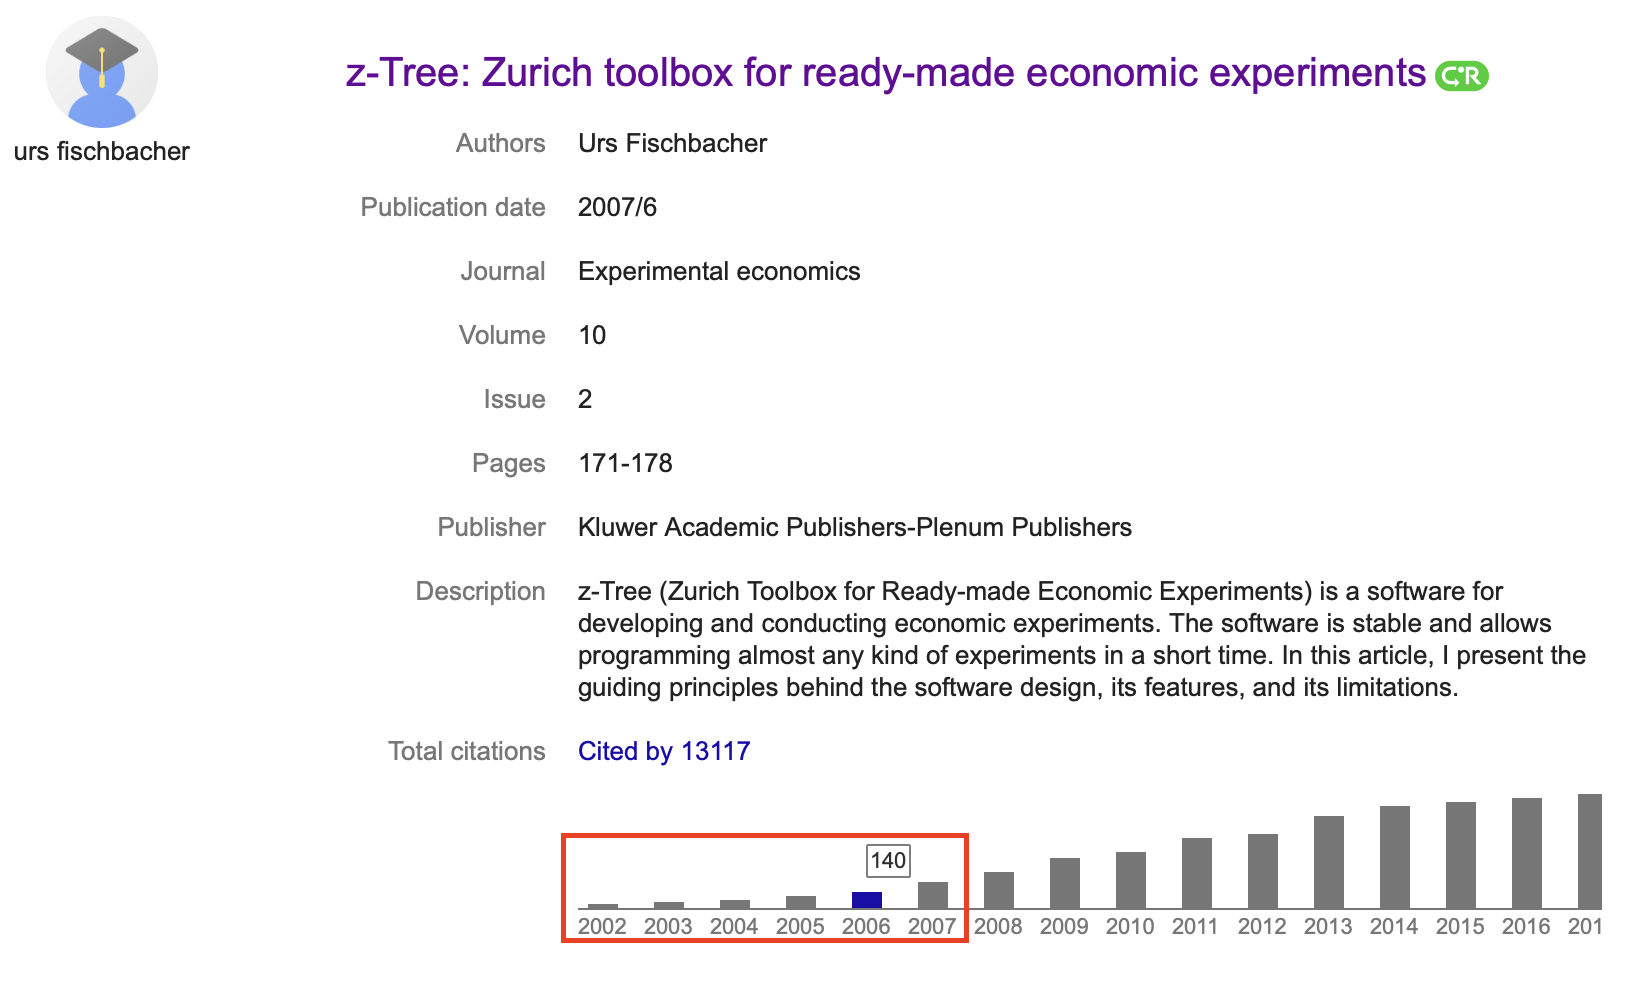
\includegraphics[width=0.8\textwidth]{figures/citation_z_tree.png}
  \caption{Nombre de citation par années de l'article de référence de z-Tree, source : Google Scholar}
  \label{fig:graph_citation_z_tree}
\end{figure}


Turocy, dit d'ailleurs dans son entretien\footnote{A la page 23}, s'être explicitement inspiré de Fischbacher et de ce modèle de \textit{citeware} pour Gambit. Ce qui permet à l'article de référence de cumuler plus de 600 citations en 2025, là aussi l'article le plus mentionné de Turocy.

L’article de référence sur z-Tree \cite{fischbacherz-TreeZurichToolbox2007} cumule ainsi, en 2025, plus de 13 000 citations, ce qui en fait de très loin la publication la plus citée d’Urs Fischbacher. Si le nombre de citations est souvent décrié par la communauté scientifique pour évaluer l'impact d'un article de recherche, une telle ampleur a nécessairement renforcé la visibilité et la reconnaissance de son auteur : c’est bien son travail de programmation qui se trouve ici crédité et valorisé.
Théodore Turocy explique d’ailleurs dans son entretien\footnote{Entretien avec Turocy\cite{turocyInterviewTheodoreTurocy2024}, p. 23} s’être explicitement inspiré de Fischbacher et de ce modèle de \textit{citeware} pour Gambit. L’article de référence du logiciel cumule ainsi, en 2025, plus de 600 citations — devenant aussi la publication la plus citée de Turocy. Ce parallèle montre combien le dispositif de \textit{citeware} constitue une stratégie efficace pour transformer un travail de programmation, difficile à valoriser, en une contribution reconnue dans le champ académique.

En somme, l’histoire de ces logiciels met en évidence un décalage structurel : bien qu’ils constituent des instruments essentiels pour certains domaines de la recherche en économie, ils peinent à être pleinement reconnu auprès des institutions. Leur émergence dépend souvent d’initiatives individuelles ou de financements circonstanciels, et leur maintien repose sur le volontarisme de leurs concepteurs, plus que sur des dispositifs pérennes. Financièrement, ils sont fragilisés par la dépendance à des subventions temporaires ou à des arrangements ad hoc difficiles à prolonger ; académiquement, ils souffrent d’un manque de reconnaissance, la programmation étant encore perçue comme une activité technique et secondaire, en marge de la "vraie" production scientifique que seraient les articles théoriques ou empiriques. Cette double contrainte, précarité matérielle et faible valorisation académique, contribue à expliquer pourquoi certains logiciels, pourtant centraux dans la transformation des pratiques économiques, peinent à s’inscrire durablement dans l’histoire officielle de la discipline.




\section{Postérité et devenir des logiciels}


La postérité des logiciels étudiés est contrastée. Certains continuent d’être diffusés et utilisés, d’autres ne subsistent plus qu’à travers leur rôle fondateur dans la littérature, et d’autres encore connaissent un maintien limité grâce à l’engagement de leurs concepteurs.

La suite logicielle issue de PcGive, développée par David Hendry et Jurgen Doornik, continue d’être diffusée commercialement par Timberlake Consultants en 2025. La dernière mise à jour date de juin 2024 (version 9.3), comme l’indique le site de Jurgen Doornik\url{https://www.doornik.com}. Une conférence des usagers d’OxMetrics s’est également tenue à Oxford les 3 et 4 avril 2025, toujours selon cette source. Elle demeure encore utilisée et mentionnée dans certains articles de recherches publiés par Hendry et Doornik\cite{castleSelectingModelForecasting2021} \cite{castleDetectingBreaksTrends2025}, en particulier en économétrie des séries temporelles. Toutefois, son statut de quasi-standard des années 1990 est progressivement concurrencé par des logiciels plus largement adoptés. Il reste difficile d’évaluer le nombre d’utilisateurs actifs en 2025, mais un constat ressort des recherches effectuées : aucun programme d’enseignement de l'économétrie récent (au cours des deux ou trois dernières années) dans les grandes universités occidentales ne fait mention de PcGive ou d’OxMetrics. Cette absence dans la formation initiale suggère que la communauté d’utilisateurs se réduit, en contraste avec la large diffusion de logiciels concurrents comme SAS, Stata, EViews ou R.

WinSolve connait un destin plus limité. La dernière version stable (4.0) date de 2007. Dans son entretien, Richard Pierse indique avoir continué à intervenir ponctuellement sur le code jusqu’en 2021, mais le logiciel n’est plus véritablement maintenu depuis. Il est utilisé pendant un temps dans certaines banques centrales et laboratoires, mais ne réussi pas à s’imposer durablement face à des environnements de modélisation macroéconomique plus flexibles comme Dynare. Sa trajectoire illustre la difficulté des logiciels dépendant d’un individu isolé à se maintenir dans le temps.

z-Tree constitue l’un des cas les plus durables. Il est conçu en 1995 et diffusé à l’international dès la fin des années 1990, il s'impose comme le standard de l’économie expérimentale. Sa robustesse et sa simplicité d’utilisation expliquent ce succès, mais il est aujourd’hui concurrencé par de nouvelles solutions, plus adaptées à l'ère du numérique. O-tree, une plateforme open source basée sur le web, est l'alternative la plus notable, car elle permet de mener des expériences en ligne et de configurer les expériences en utilisant le langage Python, bien plus connu et répandu que le langage z-Tree, spécifique à ce logiciel. D'autres variantes, comme z-Tree Unleashed, cherchent à prolonger l'outil original en repoussant ses limites techniques via le web. Bien que z-Tree conserve une position solide dans les laboratoires, son règne est désormais contesté par ces nouvelles solutions, qu'il a inspiré, conçues pour l'expérimentation en ligne.


Après avoir survécu de longues années grâce au volontarisme de Theodore Turocy, Gambit connaît aujourd’hui un renouveau partiel grâce à son intégration dans le projet "Automated analysis of strategic interactions" financé par l’Alan Turing Institute, notamment dans le domaine de l’intelligence artificielle et des agents autonomes. Son usage en économie reste limité, mais sa pertinence pour la modélisation computationnelle des agents lui confère une seconde vie, désormais plus souvent dans les cercles académiques de la théorie des jeux appliquée à d'autres disciplines que l'économie.


Sugarscape laisse une empreinte intellectuelle considérable, mais son existence logicielle est éphémère. Développé sur Macintosh, il est resté peu diffusé à l’époque, utilisé presque exclusivement par Epstein et Axtell. Après la publication de Growing Artificial Societies en 1996, le logiciel n’est pas maintenu, mais son influence se prolonge par la diffusion de la méthode de simulation multi-agents. Plusieurs environnements reprennent ses principes, notamment NetLogo, qui permet de reproduire les modèles originaux (comme celui des chasseurs-cueilleurs décrit par Epstein et Axtell), ainsi que MASON et Repast. Sugarscape est plus cité qu’utilisé : son importance tient à son rôle séminal dans l’ABM plutôt qu’à une trajectoire propre comme logiciel.


Ces différents destins soulignent que la postérité d’un logiciel ne dépend pas seulement de sa valeur scientifique initiale, mais aussi de son modèle de diffusion (open source ou commercial) et de sa capacité s’adapter aux évolutions techniques. Certains, comme Sugarscape, survivent comme références intellectuelles plus que comme outils utilisés ; d’autres, comme z-Tree ou OxMetrics, continuent à être employés mais sous la pression de la concurrence.\\





L’examen des logiciels développés par les programmeurs-économistes met en évidence un ensemble de traits communs et de contrastes qui permettent de mieux comprendre la place de l’informatique dans la discipline. Leur genèse répond presque toujours à un besoin local : faciliter l’enseignement de l’économétrie, résoudre des modèles macroéconomiques complexes, stabiliser des expériences de laboratoire ou encore explorer des phénomènes sociaux nouveaux à travers la simulation. Ces logiciels portent la marque de la débrouillardise et du pragmatisme de leurs concepteurs, qui bricolent avec les moyens techniques disponibles pour répondre à une contrainte immédiate.
Certains de ces outils ont ensuite dépassé leur fonction initiale pour devenir de véritables instruments heuristiques. Sugarscape et Gambit, en particulier, illustrent comment la simulation computationnelle peut ouvrir de nouveaux champs de recherche. Dans ces cas, la programmation ne se limite pas à exécuter des routines : elle devient une manière d’expérimenter, de découvrir et de reformuler les standards de l’explication économique.

Mais ces trajectoires sont traversées par des difficultés récurrentes. Le développement de logiciels confronte les chercheurs à des obstacles techniques lourds — choix des langages, contraintes de mémoire, conception d’interfaces ou stabilité des réseaux — qui exigent une expertise rarement valorisée par la discipline. Sur le plan institutionnel, les concepteurs se heurtent à la précarité du financement et à une reconnaissance académique limitée. Les revues hésitent à publier des articles centrés sur l’architecture logicielle, et les carrières des programmeurs-économistes pâtissent du temps consacré à ces tâches jugées « techniques ».

Enfin, l’analyse de la postérité de ces logiciels révèle des trajectoires contrastées. Certains, comme z-Tree ou PcGive/OxMetrics, se sont imposés comme des standards, tout en étant progressivement concurrencés par des alternatives. D’autres, comme WinSolve ou Gambit, ont connu une diffusion limitée ou intermittente, tributaires du volontarisme de leurs créateurs. D’autres encore, comme Sugarscape, ont davantage survécu comme références intellectuelles que comme instruments effectivement utilisés. Cette diversité des devenirs illustre la tension constante entre l’utilité pratique de ces logiciels, leur fragilité technique et leur faible reconnaissance institutionnelle.\\




Après avoir retracé l’histoire des logiciels conçus par les programmeurs-économistes et les difficultés récurrentes auxquelles ils se sont heurtés, la suite de ce travail portera sur l'analyse de leurs spécifités. Le chapitre suivant analysera plus particulièrement comment l'histoire de l'informatique et le contexte d'apprentissage de l'informatique ont produits de tels logiciels. Nous nous intéresserons ensuite à l'évolution des outils informatique de l'économiste qui permettent l'avénement d'économistes-programmeurs.